\chapter{Software Developed}
\label{chapter:software_developed}
During this project, software applications were created simultaneously with the development of hardware logic components. The author first developed software for communication with the \textit{IOb-SoC} through serial. Secondly, he programmed an application for hardware verification that used open-source logic simulators. Thirdly, he wrote firmware that could test and run interrupt routines. Fourth, he adapted and built the needed software/firmware to execute an \acrlong{os} on the \acrshort{soc} developed. Finally, the author wrote multiple Makefiles that facilitated user interaction and further development.

Some software developed was not mandatory to get a full-fledged \acrlong{os} to work with the \acrlong{soc} designed. The author worked on complementary software because it facilitates project development. Furthermore, the additional software allows the \textit{IOb-SoC} platform to support more features.

In this chapter, the software developed will be analysed. The new \textit{Python} \textit{Console} and the new simulation system were already implemented on the upstream \textit{IOb-SoC} template. Other developers are already using this software. Moreover, the \textit{IObundle} developers using it have already been improving the software.

Developers write new Makefiles while developing new hardware and software tools. In this project, the author based some of the new Makefiles on existing \textit{IOb-SoC} Makefiles. In contrast, the author wrote other Makefiles from scratch. The Makefiles help to automate the build processes and simplify the \acrshort{soc} usage.

\section{\textit{Python} \textit{Console}}
\label{section:pyhton_console}
The \textit{Console} is a program that runs on the user computer and communicates with the board where the \textit{IOb-SoC} is implemented using an \textit{RS-232} connection. Initially the \textit{IOb-SoC} had a \textit{Console} written in \textit{C} programming language. One of the first tasks developed was translating the \textit{Console} program to \textit{Python}.

The \textit{C} \textit{Console} uses a set of open-source functions present on an external file that \textit{IObundle} developers found to read/write to the serial port. The \textit{Python} program uses the \textit{PySerial} library, which provides ready-made communication functions like those in the original \textit{C} code. Using \textit{PySerial} is better because the community regularly maintains and updates \textit{PySerial}. \textit{PySerial} provides additional features, is less prone to have bugs, and communication is more trustworthy compared with the \textit{C} functions.

One of the reasons for translating the \textit{Console} program was to integrate an existing Ethernet controller already written in \textit{Python}. \textit{Python} can easily exploit feature like files, sockets and other \acrfull{os} functionalities.

Users can use the \textit{Python} \textit{Console} program in two different modes: locally working with simulators or communicating with a board running \textit{IOb-SoC}. The program mode can be choose when calling the \textit{Console} through adding \enquote{-L} or \enquote{--local} to the invoking arguments. Working in different modes is an additional feature to the original \textit{Console} program. The \textit{C} \textit{Console} could only works with the \acrshort{fpga} board. When the \textit{Console} is run in board mode a physical implementation of \textit{IOb-SoC} runs on the board and communicates with \textit{Console} through a \textit{RS-232} serial connection. If the \textit{Console} is called with the \enquote{-L} or \enquote{--local} augment it will communicate with the simulator. The communication with the hardware simulation is identical to the one with the board. They exchange the same messages. When communicating with the simulator, the \textit{Console} uses files to send and receive data from the \textit{IOb-SoC} hardware simulation. When stating, the \textit{Console} program creates two empty files in the simulation directory. The \enquote{cnsl2soc} is used to send messages from the \textit{Console} to the \acrshort{soc}. The \enquote{soc2cnsl} is used by the \textit{Console} to receive messages from the \acrshort{soc}. Both files only contain one byte at a time. Whether the files are empty or not is used to synchronise the simulation with the \textit{Console}. After reading from one of the files, the simulation or the \textit{Console} program has to empty the respective file.

How the code is structured is very similar to how it was on the \textit{C} \textit{Console} program. It starts by defining the parameters that influence message identifiers and serial communication (for example, the number of bits per byte, the parity and the number of stop bits). When the program enters its primary function, it starts a loop where it waits for an available byte to read, either from the serial port or the file, depending on the \textit{Console} execution mode. After receiving the byte from the \acrshort{soc}, it computes what type of message it is. In figure \ref*{fig:console_flow} the reader can see the \textit{Console} program flowchart.

\begin{figure}[!ht]
    \centering
    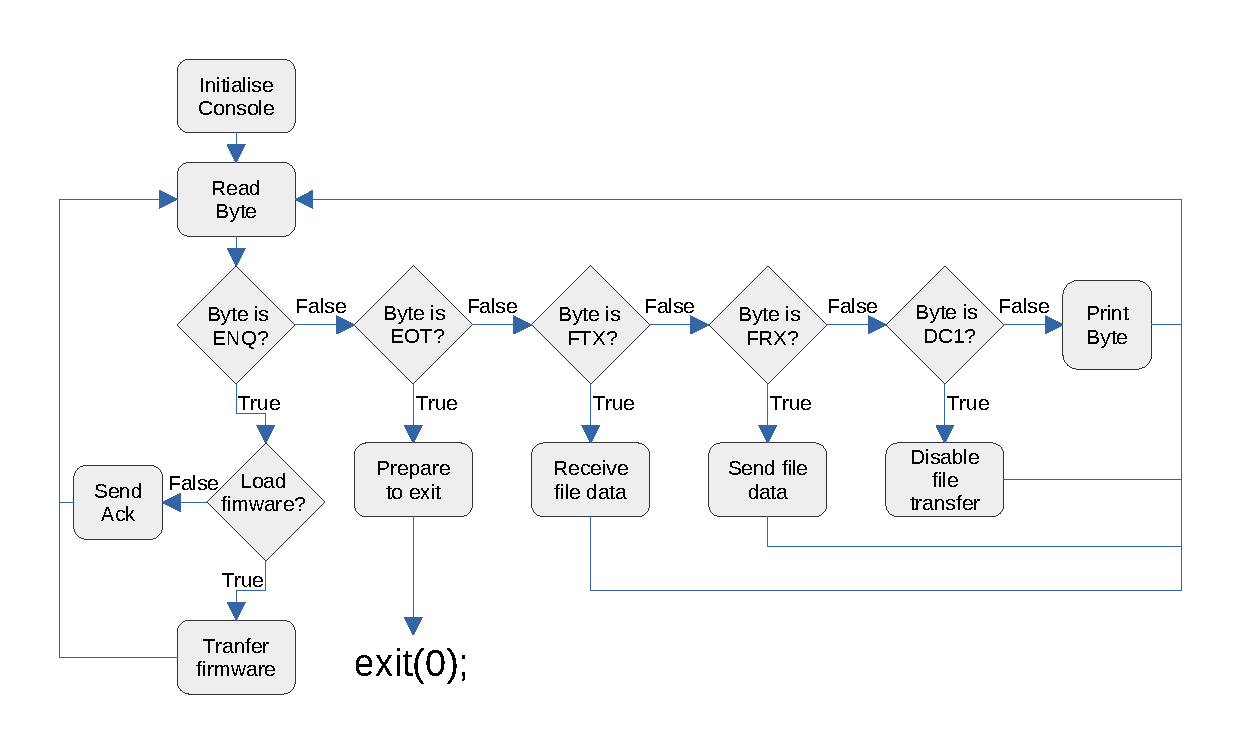
\includegraphics[width=\textwidth]{console_flow.pdf}
    \caption{\textit{Console} program flowchart.}
    \label{fig:console_flow}
\end{figure}

The program exits successfully if the byte received is an \acrlong{eot} (\acrshort{eot} = 04, \acrshort{ascii} value in hexadecimal). If the byte received is an \acrlong{enq} (\acrshort{enq} = 05, \acrshort{ascii} value in hexadecimal), the program checks if it was the first time it received an enquiry. If it was, it could have one of either behavior: if the program was called with an argument equivalent to \enquote{-f}, meaning that there is a firmware that should be uploaded to the \textit{IOb-SoC}, the \textit{Console} sends a \acrlong{frx} message (\acrshort{frx} = 08, value in hexadecimal) to the \textit{IOb-SoC}; if there is not a firmware file to send then the \textit{Console} responds to the \textit{IOb-SoC} with an \acrlong{ack} (\acrshort{ack} = 06, \acrshort{ascii} value in hexadecimal). If the \textit{Console} receives a \acrlong{ftx} message (\acrshort{ftx} = 07, value in hexadecimal), it will run a function that will receive any file sent from the \textit{IOb-SoC} to the computer and save it under the directory where it is running. If the \textit{Console} receives a \textit{Send a file request} message, it will run a function that will send any file requested from the \textit{IOb-SoC} to it. Any other byte received will be printed onto the stdout.

The FRX and the FTX bytes are specific to the \textit{IOb-SoC} platform software. Being platform-specific could cause a problem when using external software that does not attribute the same meaning to their respective values. To solve this problem a meaning for the \acrlong{dc1} (\acrshort{dc1} = 11, \acrshort{ascii} value in hexadecimal) byte was created. When receiving a \acrshort{dc1} byte the \textit{Console} deactivates all platform-specific meanings for the respective bytes. This means that after receiving a \acrshort{dc1} byte stops associating the value 0x07, 0x08, 0x11 to FTX, FRX and \acrshort{dc1} respectively. 

An example of how to call the \textit{Console} to communicate with the simulation and send the firmware to the \textit{IOb-SoC} when it starts would be \ref{lst:call_console}. The \enquote{\&} at the end means that the \textit{Console} program will run in the background. Consequently, it allows other programs to run while the \textit{Console} executes.

\begin{lstlisting}[language=make, caption={Call \textit{Console} program}, label=lst:call_console]
    CONSOLE_CMD=$(CONSOLE_DIRECTORY)/console -L -f &
\end{lstlisting}

\section{\textit{IOb-SoC} Simulation}
\label{section:simulation}
In order to support the new \textit{Console} simulation mode a new \textit{IOb-SoC} verification mechanism had to be developed. Verification is an important concern when developing hardware. As a result, it is unnecessary to synthesise and flash the hardware to an \acrshort{fpga} every time a developer wants to test a new feature. A correct and precise verification saves time.

%might be SOA?
The original simulation testbench was written in \textit{Verilog} \acrshort{hdl}. The simulation testbench in \textit{Verilog} is a hardware module without any input or output signals. In this hardware module it was instantiated the \acrfull{uut}, a testing \acrshort{uart} and the \acrshort{ddr} memory. The \acrshort{uut} was equivalent to the \acrshort{soc} tested during the simulation. The testbench used the test \acrshort{uart} to simulate an RS232 interface with the \acrshort{uut}. The \acrshort{ddr} memory would only be instantiated when the \acrshort{soc} used an external \acrshort{dram} memory.

Inside the initial block is where the developers described the simulation behaviour. The testbench runs the initial block in a \textit{Verilog} hardware module only once when it instantiates the module. The original testbench starts by resetting the \acrshort{soc}. Resetting the \acrshort{soc} initialises the hardware registers to their reset values. The testbench configures the test \acrshort{uart} to communicate with the \acrshort{soc} \acrshort{uart}. Developers must configure both \acrshort{uart}s to use the same baud rate. After the initial setup, the simulation enters an \enquote{infinite} loop.

The testbench uses the \enquote{infinite} loop to send and receive bytes from the \acrshort{soc} until the simulation finishes. Thus the loop is not infinite, but the loop condition is always true. There exists a file called \enquote{cpu\_tasks.v} that assists the testbench and contains multiple \textit{Verilog} tasks.  \textit{Verilog} tasks are similar to \textit{C} functions. The tasks in \enquote{cpu\_tasks} are used to read and write to the test \acrshort{uart}. The testbench uses a task to get a byte from the \acrshort{soc} that waits for the UART to have an available byte to read and reads it. Then, the testbench proceeds to process the received byte. If the received byte was a control byte, the testbench responds to the \acrshort{soc} by writing to the test \acrshort{uart}. If not, the console prints the received byte to the stdout in the terminal. The control bytes could be an \acrfull{enq}, \acrfull{eot}, \acrfull{ftx} or \acrfull{frx}.

The simulation testbench would successfully end when it received an \acrshort{eot} byte from \acrshort{soc}. The simulation would end abruptly when a trap notification was received. The \enquote{trap} signal was enabled (set to '1') when the \acrshort{cpu} encountered an illegal instruction.
%end of SOA? If this is state of the art, I must describe the control signals.

When the old testbench interacted with the test \acrshort{uart} it emulated the \textit{Console} program. Consequently, every time developers updated the \textit{Console}, the simulation also had to be updated. Hence, the idea was to create a testbench that allowed the simulator to interact with the \textit{Console} program. The new simulation now has the advantage of mostly using the same \textit{Console} program as when the \textit{IOb-SoC} is implemented in an \acrshort{fpga}.

The new verification software separates the previous simulation testbench into two parts. One of the parts is a hardware top module, and all hardware logic simulators use the hardware top module. The other is the simulation testbench, which is specific to each simulator. The simulation testbench interacts with the \acrshort{uut} through the hardware top module. The new testbench does not use the \enquote{trap} signal; only the old simulation uses it. Since the author swapped the \acrshort{cpu}, the \acrshort{cpu} no longer uses the trap signal to notify if something went wrong. Now the \acrshort{cpu} handles trap exceptions on its hardware. Furthermore, they might not always mean the end of the execution or failure. The reader can see a sketch of the verification software in figure~\ref{fig:uut_top_hw}.

\begin{figure}[!ht]
    \centering
    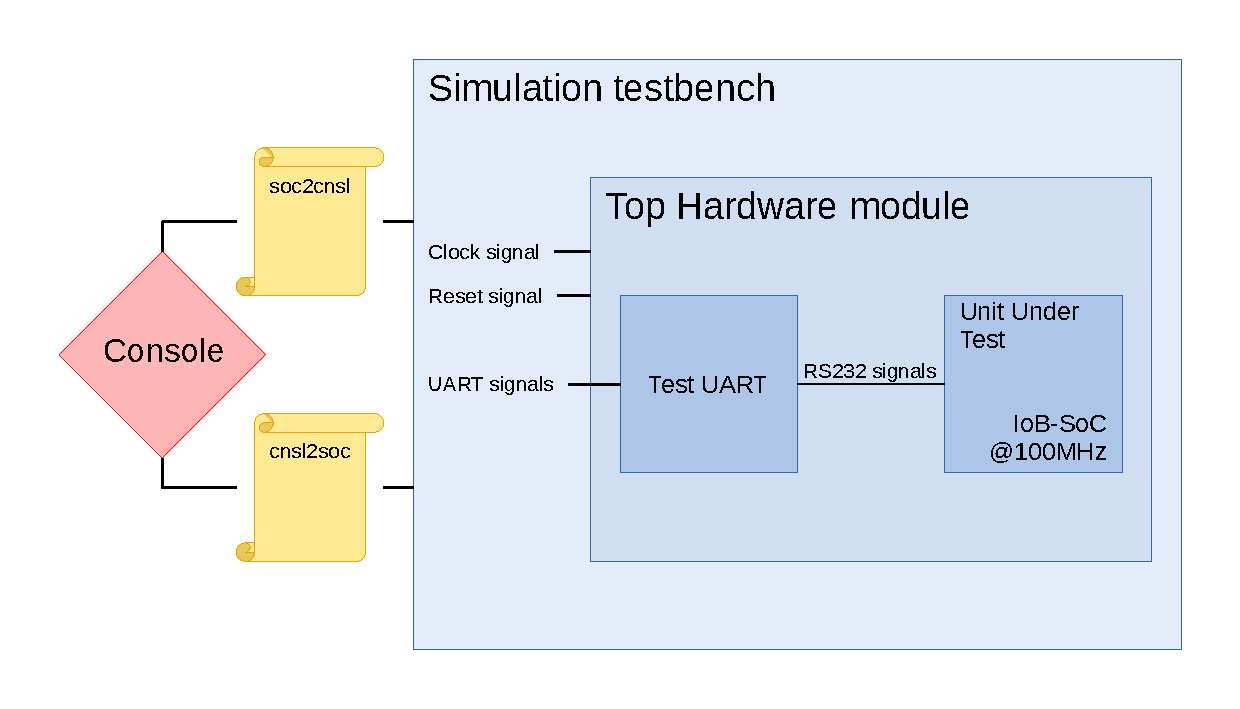
\includegraphics[width=\linewidth]{uut_top_hw.pdf}
    \caption{Simulated hardware interfaces.}
    \label{fig:uut_top_hw}
\end{figure}

\subsection{Top Hardware module}
This top module creates a \textit{verilog} wrapper of the \acrfull{uut}. The \acrshort{uut} interacts with the different hardware logic simulators through this wrapper. Developers can never implement the top hardware module as real hardware. Developers only use this module in simulation as software.

The top module file adapts a part of the previous \textit{verilog} simulation testbench. In the top module, the simulation only uses the initial block to obtain the system simulation signals waves. Developers can use these waves to debug the behaviour of the simulated hardware components. The user can define if the signal waves should be saved or not. The top hardware module instantiates the \acrfull{uut}, a testing \acrshort{uart} and the \acrshort{ddr} memory. The \acrshort{uut} shares an interface with the test \acrshort{uart} and the \acrshort{ddr} memory.

The test \acrshort{uart} is connected to the \acrshort{soc} under test through the \enquote{rx} and \enquote{tx} pins. The \enquote{rx} pin in the \acrshort{soc} is connected to the \enquote{tx} pin in the test \acrshort{uart} and is used to send information from the test \acrshort{uart} to the\acrshort{soc}. Similarly, the \enquote{tx} pin in the \acrshort{soc} is connected to the \enquote{rx} pin in the test \acrshort{uart} and is used to send information from the the\acrshort{soc} to the test \acrshort{uart}. The interface between the \acrshort{soc} and the test \acrshort{uart} simulates an RS232 connection.

The author described the input and output signals with which the top hardware module integrates with the simulation testbench in table~\ref{tab:input_output_top_simulation}.

\begin{table}[!ht]
    \centering
    \begin{tabular}{|l|l|l|l|}
    \hline
    \textbf{Port} & \textbf{Width} & \textbf{Direction} & \textbf{Description}                                                                                                                    \\ \hline
    clk           & 1              & input              & \begin{tabular}[c]{@{}l@{}}The system clock signal generated in\\  the simulation testbench.\end{tabular}                               \\ \hline
    rst           & 1              & input              & \begin{tabular}[c]{@{}l@{}}The system reset signal generated in\\  the simulation testbench.\end{tabular}                               \\ \hline
    trap          & 1              & output             & Not used.                                                                                                                               \\ \hline
    uart\_valid   & 1              & input              & \begin{tabular}[c]{@{}l@{}}Used for the simulation testbench to\\  make a write/read request to the\\  test UART.\end{tabular}          \\ \hline
    uart\_addr    & 32             & input              & \begin{tabular}[c]{@{}l@{}}Indicates the test UART register to \\  which the simulation testbench\\  wants to write/read.\end{tabular}  \\ \hline
    uart\_wdata   & 32             & input              & \begin{tabular}[c]{@{}l@{}}Data that the simulation testbench\\  wants to write in the test UART.\end{tabular}                          \\ \hline
    uart\_wstrb   & 4              & input              & \begin{tabular}[c]{@{}l@{}}Select bytes from uart\_wdat to write\\  to the test UART register.\end{tabular}                             \\ \hline
    uart\_rdata   & 32             & output             & \begin{tabular}[c]{@{}l@{}}Data sent from the test UART to the\\  simulation testbench as a response\\  to a read request.\end{tabular} \\ \hline
    uart\_ready   & 1              & output             & \begin{tabular}[c]{@{}l@{}}Used by the test UART to indicate\\  that the response to a write/read\\  is ready.\end{tabular}             \\ \hline
    \end{tabular}
    \caption{Inputs and outputs of the top hardware module used in the simulation.}
    \label{tab:input_output_top_simulation}
\end{table}

Although in this project \acrshort{soc} the \textit{IOb-UART} in the \acrfull{soc} was swapped for the \textit{UART16550} in the simulation testbench the \textit{IOb-UART} is still used. If the \acrshort{clint} unit used a \acrlong{rtc} derived from the board, the \acrlong{rtc} should be added in the simulation testbench. When added to the testbench, the top hardware module would have an additional input for the \acrshort{rtc}.

\subsection{Simulation Testbench}
The author developed two simulation testbench during this project. One testbench was written in \textit{Verilog} and is used by some simulators as for example \textit{Icarus Verilog} and \textit{xcelium}. Another testbench was written in \textit{C} programming language and is used by the \textit{Verilator} hardware logic simulator.

The new \textit{Verilog} simulation testbench developed instantiates only the top hardware module. At the beginning of the testbench module, the testbench generates the system clock. If the development board had a \acrlong{rtc}, the testbench should also generate the \acrshort{rtc} signal. The reader can see the creation of both these signals in the code snippet~\ref{lst:clk_rtc_gen}. The \acrshort{rtc} signal does not apply to the \acrshort{soc} developed in the end, so the developer wrote the code that generated it as a comment.

\begin{lstlisting}[language=Verilog, caption={System clock and \acrshort{rtc} generation in \textit{Verilog}.}, label=lst:clk_rtc_gen]
    parameter realtime clk_per = 1s/`FREQ;
    //parameter realtime rtc_per = 1s/`RTC_FREQ;
 
    //clocks
    reg clk = 1;
    always #(clk_per/2) clk = ~clk;
    //reg rtc = 1;
    //always #(rtc_per/2) rtc = ~rtc;
\end{lstlisting}

The new testbench initial block starts by executing the same procedure as the previous testbench. It first sends a reset signal to the system and initialises the test \acrshort{uart}. The testbench initialises the test \acrshort{uart} with a specified baud rate. Before entering an \enquote{infinite} loop, the new testbench will check if the file used to communicate with the \textit{Console} exists. This file is called \enquote{soc2cnsl}. The file \enquote{soc2cnsl} should have been created by the \textit{Console} program, executed before the testbench. If this file does not exist, the simulation will end abruptly. When the simulation ends unsuccessfully, it informs the user of its cause. The \textit{Console} creates the \enquote{cnsl2oc} file simultaneously with the \enquote{soc2cnsl}, but the testbench will only check if that file exists inside the loop. The testbench uses the \enquote{cnsl2oc} file to receive messages from the console. While it uses the \enquote{soc2cnsl} file to send messages to the console.

The \enquote{infinite} loop is a while statement whose loop condition is always true, similar to the old testbench. Inside the loop the testbench will read the test \acrshort{uart} \enquote{rx} ready register and the \enquote{tx} ready register until either one of them is enabled (set to '1'). As can be seen in the code snippet~\ref{lst:rx_tx_read}. The \enquote{cpu\_uartread} task is the same task used in the previous testbench to read from the test \acrshort{uart}. The first argument of the task is the address of the \acrshort{uart} register, which is to read. The second argument is the variable that saves the value of the register.

\begin{lstlisting}[language=Verilog, caption={Read the test \acrshort{uart} \enquote{rx} ready register and the \enquote{tx} ready register.}, label=lst:rx_tx_read]
    while(!rxread_reg && !txread_reg) begin
        cpu_uartread(`UART_RXREADY_ADDR, rxread_reg);
        cpu_uartread(`UART_TXREADY_ADDR, txread_reg);
    end
\end{lstlisting}

After exiting the while, the testbench executes code depending on the register's value. If the variable used to store the \enquote{rx} ready register value (\enquote{rxread\_reg}) is true the testbench will read a byte sent by the \acrshort{soc} under test and send it to the \textit{Console}. To do that, it will first open the \enquote{soc2cnsl} file in reading mode and check if it is empty. If the file is empty, the testbench will close the file and read the value stored in the test \acrshort{uart} \enquote{rx} data register. Then the testbench will reopen the \enquote{soc2cnsl} file in write mode and write the value read. After writing to the file the testbench will clear the \enquote{rxread\_reg} and close the \enquote{soc2cnsl} file. If the file is not empty, the testbench will just close it and verify if it is empty again in the next loop. The program logic is seen in code snippet~\ref{lst:write2cnsl}. The simulation clock signal only advances when the testbench reads or writes to the test \acrshort{uart}. By not clearing the \enquote{rxread\_reg} variable, the testbench will wait until the \enquote{soc2cnsl} file is empty before proceeding with the simulation.

\begin{lstlisting}[language=Verilog, caption={Write byte from \acrshort{soc} to \textit{Console}.}, label=lst:write2cnsl]
    if(rxread_reg) begin
        soc2cnsl_fd = $fopen("soc2cnsl", "r");
        n = $fgets(cpu_char, soc2cnsl_fd);
        if(n == 0) begin
            $fclose(soc2cnsl_fd);
            cpu_uartread(`UART_RXDATA_ADDR, cpu_char);
            soc2cnsl_fd = $fopen("soc2cnsl", "w");
            $fwriteh(soc2cnsl_fd, "%c", cpu_char);
            rxread_reg = 0;
        end
        $fclose(soc2cnsl_fd);
    end
\end{lstlisting}

If the variable used to store the \enquote{tx} ready register value (\enquote{txread\_reg}) is true the testbench will read a byte sent by the \textit{Console} and send it to the \acrshort{soc} under test. In order to do that, the testbench will first try to open the \enquote{cnsl2soc} file in reading mode. If opened successfully, it would proceed, read the first byte in the file, and save it in the \enquote{cpu\_char} variable. When the read is successful, the testbench will write the \enquote{cpu\_char} to the test \acrshort{uart}. Then the testbench will close the \enquote{cnsl2soc} file and reopen it in write mode. This way, the file will be truncated to have 0 bytes. If the read was unsuccessful, it means the \textit{Console} does not want to send aa Byte to thee \acrshort{soc}. Then the testbench will just ignore that part of the code. Finally the \enquote{cnsl2soc} file is closed and the \enquote{txread\_reg} variable is cleared. The simulation finishes if the testbench cannot open the \enquote{cnsl2soc} file. Normally this means that the simulation was successful. The \enquote{cnsl2soc} file is deleted by the \textit{Console} program when the \acrshort{soc} send a \acrfull{eot} Byte. The \acrshort{eot} Byte means the \acrshort{soc} has finished running the firmware.

\begin{lstlisting}[language=Verilog, caption={Write byte from \textit{Console} to \acrshort{soc}.}, label=lst:write2soc]
    if(txread_reg) begin
        cnsl2soc_fd = $fopen("cnsl2soc", "r");
        if (!cnsl2soc_fd) begin
            $finish;
        end
        n = $fscanf(cnsl2soc_fd, "%c", cpu_char);
        if (n > 0) begin
            cpu_uartwrite(`UART_TXDATA_ADDR, cpu_char, `UART_TXDATA_W/8);
            $fclose(cnsl2soc_fd);
            cnsl2soc_fd = $fopen("./cnsl2soc", "w");
        end
        $fclose(cnsl2soc_fd);
        txread_reg = 0;
    end
\end{lstlisting}

The \textit{Verilator} testbench is similarly structured to the \textit{Verilog} testbench. The code in the initial block written for the \textit{Verilog} testbench also applies to the \textit{Verilator} testbench. The code only had to be translated from \textit{Verilog} to \textit{C} language. One of the main differences between the \textit{Verilator} testbench and the \textit{Verilog} testbench is how the simulators generate the clock signals. \textit{Verilator} executes the simulation through cycles. Executing the simulation through cycles means that the testbench controls the time advancement. With that in mind, the author implemented a global variable that saved the current time and created a function that advances time. The reader can see the function in code snippet~\ref{lst:verilator_timer}. The function, when executed, advances the number of nanoseconds passed as an argument. Every nanosecond passed, a cycle has passed, and \textit{Verilog} verifies the state of the \acrfull{uut}. The system clock signal has to change value every half of the clock period. If the hardware used a \acrshort{rtc}, the \acrshort{rtc} value would have to change every half of the defined \acrlong{rtc} period.

\begin{lstlisting}[language=C, caption={\textit{Verilator} Timer function.}, label=lst:verilator_timer]
    void Timer(unsigned int ns){
        for(int i = 0; i<ns; i++){
            if(!(main_time%(CLK_PERIOD/2))){
                uut->clk = !(uut->clk);
            }
            //if(!(main_time%(RTC_PERIOD/2))){
            //  uut->rtc_in = !(uut->rtc_in);
            //}
            uut->eval();
            main_time += 1;
        }
    }
\end{lstlisting}

In the previous testbench, the \textit{IObundle} developers had developed tasks that initialise the test \acrshort{uart} and read/write to the registers. The new \textit{Verilog} testbench uses the tasks developed by \textit{IObundle}. For the \textit{Verilator} testbench those functions had to be rewritten in \textit{C}. The test \acrshort{uart} initialization starts by resetting the test \acrshort{uart} hardware by writing to the \enquote{softreset} register. Then it writes to the \enquote{div} register the value needed for the \acrshort{uart} to work with the defined \acrshort{soc} frequency and baud rate. Finally it enables the \enquote{rx} and \enquote{tx} communication by writing '1' to the \enquote{rxen} and \enquote{txen} registers respectively. The initialization function can be seen in code snippet~\ref{lst:init_uart}.

\begin{lstlisting}[language=C, caption={Function to initialize the test \acrshort{uart}.}, label=lst:init_uart]
    void inituart(){
        //pulse reset uart
        uartwrite(UART_SOFTRESET, 1, UART_SOFTRESET_W/8);
        uartwrite(UART_SOFTRESET, 0, UART_SOFTRESET_W/8);
        //config uart div factor
        uartwrite(UART_DIV, int(FREQ/BAUD), UART_DIV_W/8);
        //enable uart for receiving
        uartwrite(UART_RXEN, 1, UART_RXEN_W/8);
        uartwrite(UART_TXEN, 1, UART_TXEN_W/8);
    }
\end{lstlisting}

The testbench takes two clock cycles to read a test \acrshort{uart} register. In the first clock cycle, the testbench makes a read request to the \acrshort{uart}. The testbench sets the \acrshort{uart} address signal to the address of the register that the testbench wants to read, and the \acrshort{uart} valid signal is set to '1' to make the request. In the second clock cycle, the testbench reads the response data in the \enquote{rdata} signal. The read function can be seen in code snippet~\ref{lst:read_uart}.

\begin{lstlisting}[language=C, caption={Read from the test \acrshort{uart}.}, label=lst:read_uart]
    void uartread(unsigned int cpu_address, char *read_reg){
        dut->uart_addr = cpu_address >> 2; // 32 bit address (ignore 2 LSBs)
        dut->uart_valid = 1;
        Timer(CLK_PERIOD);
        *read_reg = (dut->uart_rdata) >> ((cpu_address & 0b011)*8); // align to 32 bits
        dut->uart_valid = 0;
    }
\end{lstlisting}

The testbench has to send a write request signal to the test \acrshort{uart} to write on a \acrshort{uart} register. To make a write request the testbench as to set the \acrshort{uart} address sign, the \acrshort{uart} valid, the \acrshort{uart} \enquote{wdata} signal and the \acrshort{uart} \enquote{wstrb} signal. The testbench sets the address signal to the address of the register where it wants to write and valid to '1'. The testbench also sets the \enquote{wdata} to the data the developer wants to write on the register. Additionally, it sets the \enquote{wstrb} to indicate which Bytes from the \enquote{wdata} the developer wants to write on the register. After one clock cycle, the \acrshort{uart} completes the writing process, and the valid signal has to be set back to '0'. The write function can be seen in code snippet \ref{lst:write_uart}.

\begin{lstlisting}[language=C, caption={Write to the test \acrshort{uart}.}, label=lst:write_uart]
    void uartwrite(unsigned int cpu_address, unsigned int cpu_data, unsigned int nbytes){
        char wstrb_int = 0;
        switch (nbytes) {
            case 1:  wstrb_int = 0b01; break;
            case 2:  wstrb_int = 0b011; break;
            default: wstrb_int = 0b01111; break;
        }
        dut->uart_addr = cpu_address >> 2; // 32 bit address (ignore 2 LSBs)
        dut->uart_valid = 1;
        dut->uart_wstrb = wstrb_int << (cpu_address & 0b011);
        dut->uart_wdata = cpu_data << ((cpu_address & 0b011)*8); // align data to 32 bits
        Timer(CLK_PERIOD);
        dut->uart_wstrb = 0;
        dut->uart_valid = 0;
    }
\end{lstlisting}

\section{Interrupt Routine}
\label{section:barebones_interrupt_routine}
During the development of the \acrshort{clint} hardware unit, no firmware used the \acrshort{clint} features. The \acrshort{clint} enables the support for time or software-related interrupts. Therefore, the author needed to create a simulation testbench to test the \acrshort{clint} hardware. Moreover, the author also created bare-metal firmware that uses interrupts to understand how interrupts are used in code and handled by the \acrshort{cpu}.

The software has to write to the \enquote{MTIMECMP} register to generate a time-related interrupt. The \enquote{MTIMECMP} register address is the \enquote{MTIMECMP\_BASE} address, which is 0x4000, plus 0x08 times the core id. The core id is the \enquote{TARGET}, \acrshort{cpu} core, which is supposed to receive the interrupt notification. Since there is only one core in this project, the core id is 0. Furthermore, when writing firmware to run on the \acrshort{soc}, it is necessary to consider the \acrshort{clint} peripheral base address and add it to the \enquote{MTIMECMP} register address. For a timer interrupt to trigger after 10 seconds, the firmware has to do more than just write to the \enquote{MTIMECMP}. First, the firmware has to read the current time. A developer can obtain the current time from the \enquote{MTIME} register. Although not directly since the \enquote{MTIME} register increments with the \acrshort{clint} designed frequency, in this case 100MHz. To convert the value in \enquote{MTIME} register to seconds we know that $seconds=\frac{*(MTIME)}{frequency}$. The \enquote{MTIME} register address is obtained similarly to the \enquote{MTIMECMP} register but instead of the \enquote{MTIMECMP\_BASE}, the \enquote{MTIME\_BASE}, which is 0xbff8, is used. After reading the current time, the software calculates the value that \acrshort{cpu} needs to store in \enquote{MTIMECMP} register. The software calculates the value by adding to the current time the time waited before the \acrshort{clint} hardware triggers the interrupt. The value calculated can then be stored in the \enquote{MTIMECMP} register. When the \enquote{MTIME} register value is equal to or greater than the \enquote{MTIMECMP} register value, the timer interrupt is enabled. The pseudo-code to set up the timer interrupt is in the code snippet \ref*{lst:set_up_mtip}.

\begin{lstlisting}[language=C, caption={Set Up Timer Interrupt.}, label=lst:set_up_mtip]
    #define MTIMECMP_BASE 0x4000
    #define MTIME_BASE 0xbff8
    #define FREQ 100000000
    void set_up_mtip(time_sec){
        long long aux_value = 0; // 64-bit integer
        int core_id = 0;
        aux_value = *(MTIME_BASE+8*core_id)
        aux_value = aux_value + time_sec*FREQ;
        *(MTIMECMP_BASE+8*core_id) = aux_value;
    }
\end{lstlisting}

The \acrshort{cpu} could have readen the core id from the \acrshort{csr}, which saves its value. The \textit{RISC-V} instruction that does so is \enquote{csrr    \%0, mhartid}. An example of a C code integration would be code snippet \ref*{lst:read_mhartid}.

\begin{lstlisting}[language=C, caption={Read core id from \acrshort{csr}.}, label=lst:read_mhartid]
    static inline uint_32_t csr_read_mhartid(void) {
        uint_32_t value;        
        __asm__ volatile ("csrr    %0, mhartid"
                          : "=r" (value)  /* output : register */
                          : /* input : none */
                          : /* clobbers: none */);
        return value;
    }
\end{lstlisting}

One of the software interrupt usages is synchronising various cores in a system. When dividing the workload between cores, there might be a time when core 1 has to synchronise with core 0. Core 1 would wait until core 0 generates a software interrupt targeting core 1. This project has only one core, so this situation does not occur. Nevertheless, applications can run concurrently with multi-threading. One application could wait until a software interrupt is triggered. The \acrshort{cpu} could trigger a software interrupt targeting core 0, using another application running in core 0. The software has to write to the \enquote{MSIP} register to generate a software-related interrupt. The \enquote{MSIP} register address is the \enquote{MSIP\_BASE} address, which is 0x00, plus 0x04 times the core id. When executing the firmware, the developers must not overlook adding the \acrshort{clint} peripheral base address to the \enquote{MSIP} register. Only hardware external to the \acrshort{clint} unit can change the state of the \enquote{MSIP} register. The \acrshort{clint} hardware cannot change it internally. The pseudo-code to set up the software interrupt is in the code snippet \ref*{lst:set_up_msip}.

\begin{lstlisting}[language=C, caption={Set Up Software Interrupt.}, label=lst:set_up_msip]
    #define MSIP_BASE 0x00
    void set_up_msip(){
        int core_id = csr_read_mhartid();
        *(MSIP_BASE+4*core_id) = 1;
    }
\end{lstlisting}

After enabling an interrupt, the \acrshort{clint} sends a hardware notification. The interrupt notification has to be handled by the rest of the hardware. The \acrshort{clint} testbench and the bare-metal firmware handle the interrupt notification differently.

\subsection{CLINT simulation}
\label{subsection:clint_simulation}
The author built a simulation testbench in Verilog and another in C++ programming language to test the \acrshort{clint} hardware unit. These simulations allow the developers to test the correctness of the hardware component without connecting it to the rest of the \acrshort{soc}.

Both the testbench in Verilog and the testbench in C++ had similar behaviours. First, they would set up a timer interrupt. The testbench set the timer interrupt to trigger in $0.2*10^{-6}$ seconds. Considering that the simulation was slow, this was a reasonable time. After the timer interrupt is triggered, the simulation receives its notification and proceeds to handle the interrupt. When receiving a timer interrupt, the simulation sets up the software interrupt. The \acrshort{clint} unit notifies the testbench of an existing software interrupt in the next clock cycle. It then proceeds to disable the timer and the software interrupt. To disable the timer interrupt the \enquote{MTIMECMP} register has to be set to its maximum value, which is 0xFFFFFFFFFFFFFFFF (i.e. all 64 bits are '1'). The \enquote{MSIP} register had to be set to 0 to disable the software interrupt.

If the interrupts work correctly, there will be a message in the terminal indicating their correctness. After testing that both interrupts work as expected, the testbench can finish successfully. The simulation will always end $1*10^{-6}$ seconds after starting.

\subsection{Bare-metal firmware}
\label{subsection:interrupt_firmware}
Once the author developed the \acrshort{clint} unit, even though he knew that the \acrshort{clint} generated the interrupts through the simulation testbench, he had to test it while integrated into the \acrshort{soc}. To test the \acrshort{clint} in the \acrshort{soc} firmware that took advantage of the timer and software interrupts had to be developed.

Since the \acrshort{clint} hardware developed is compatible with \textit{RISC-V}, any firmware compatible with \textit{RISC-V} that took advantage of interrupts should work. With this in mind, the open-source bare-metal firmware made available by \textit{Five EmbedDev}~\cite{bare_metal_int}, an embedded \textit{RISC-V} blog, would be taken advantage of. The firmware could not all be used directly in \textit{IOb-SoC}. Some functions that interact with the timer in the \acrshort{clint} were adapted to the developed hardware and used. Furthermore, as a library, the firmware uses a file that implements functions that read/write to the \acrlong{csr}.

The developed firmware.c, similarly to the original \textit{IOb-SoC} firmware, starts by initializing the \acrshort{uart} and the \acrshort{clint} hardware. Then it will disable all global interrupts. To disable the global interrupts the \enquote{mstatus} \acrshort{csr}, \enquote{mie} \acrshort{csr} and the \enquote{mcause} \acrshort{csr} are cleared. After the timer interrupt is set similarly to the code in \ref{lst:set_up_mtip}. The program counter has to jump to a specific function when an interrupt occurs. The memory address of that function is saved in the \enquote{mtvec} \acrshort{csr}. Succeeding the timer interrupt set up, the respective interrupt bit can be set to '1' (i.e. enable the timer interrupt) in the \enquote{mie} \acrshort{csr}. Following this, the global interrupts can be enabled again by setting the needed bits in \enquote{mstatus} \acrshort{csr} to '1'. The bits that the firmware needs to set to '1' correspond to the machine interrupts (MSTATUS\_MIE\_BIT\_MASK). Finally, the program can wait for an interrupt to happen with the \enquote{wfi} instruction.

When an interrupt occurs, the \acrshort{cpu} calls the interrupt handler function. The interrupt handler will read the cause of the generated interrupt from the \enquote{mcause} \acrshort{csr}. After knowing the cause, the interrupt handler will act accordingly to how it was programmed. The developed firmware informs the user that a timer interrupts occurred, and it sets the \enquote{MTIMECMP} register to a higher number. The developed firmware finishes after receiving the first interrupt.

It is important to note that besides the firmware.c some alterations had to be made in the \textit{IOb-SoC} firmware.S file. In the firmware.S, the author had to set the global pointer register. The global pointer is similar to the stack pointer. The difference is that while the stack pointer points to the memory location where function variables will be stored, the global pointer points to the memory location where global variables are stored. When setting the global pointer, it is critical to write the \enquote{norelax} option in the Assembly code. Without \enquote{.option norelax}, the software will load the global pointer relative to the global pointer set in the assembly code.

\section{IOb-SoC Linux OS integration}
\label{section:linux_os_integration}
The last step in this thesis development was creating and integrating a minimal \acrfull{os} on the developed \acrfull{soc}. The minimal \acrshort{os} developed has the Linux software as its kernel. The Linux kernel allows the user applications run on the \acrshort{soc} to compile with the \textit{riscv64-unknown-linux-gnu-*} compiler. Applications compiled with \textit{riscv64-unknown-linux-gnu-*} can use the Linux system functions and drivers. Using Linux system functions and drivers allows the software developers to ignore the hardware platform where the software will run.

During the development of the \acrshort{os} to run on the \acrshort{soc}, the author had to adapt the bootloaders firmware and write the device tree describing the developed \acrshort{soc}. Additionally he had to compile the Linux kernel compatible with the \textit{VexRiscv} \acrshort{cpu} implemented on the \acrshort{soc} and create a \acrlong{rootfs}. Moreover, additional features had to be developed for the user to interact with the \acrshort{os}.

The author developed a Makefile target for each component that automates the build process. Furthermore, he created a general target called \enquote{build-OS}. \enquote{build-OS} calls all other targets and builds a full-featured minimal \acrshort{os}.

\subsection{Bootloaders}
Before running the Linux kernel software, the \acrshort{soc} has to run two bootloader firmware programs. The first firmware to execute is the stage 0 bootloader. The stage 0 bootloader , which the author refers to as \textit{iob-bootloader}, is an adaptation of the bootloader firmware used in \textit{IOb-SoC}. The second bootloader is a \textit{RISC-V} specific software called \textit{OpenSBI}.

The \textit{iob-bootloader} has to copy the developed \acrshort{os} to the external memory of the \acrshort{soc} running on the \acrshort{fpga} board. The bootloader will send a request to the \textit{Console} program asking for the binary data of the \textit{OpenSBI}, the device tree, the Linux kernel and the \acrlong{rootfs}. Each file transferred will be stored in a specific memory location. The transfer bootloader code can be seen in \ref{lst:copy_bynaries}.

\begin{lstlisting}[language=c, caption={Transfer \acrshort{os} to the \acrshort{soc} external memmory.}, label=lst:copy_bynaries]
    prog_start_addr = (char *)(EXTRA_BASE + 0x00000000);
    file_size = uart_recvfile(opensbi, prog_start_addr);
    prog_start_addr = (char *)(EXTRA_BASE + 0x00400000);
    file_size = uart_recvfile(kernel, prog_start_addr);
    prog_start_addr = (char *)(EXTRA_BASE + 0x00F80000);
    file_size = uart_recvfile(dtb, prog_start_addr);
    prog_start_addr = (char *)(EXTRA_BASE + 0x01000000);
    file_size = uart_recvfile(rootfs, prog_start_addr);
\end{lstlisting}

When finishing, the \textit{iob-bootloader} has to ensure that it clears all of the \acrshort{cpu}’s function argument registers. The bootloader has to write '0' to a function argument register to clear it. An example of clearing the first function argument register is seen in listing \ref{lst:clear_a_reg}. There are in total eight function argument registers in a \textit{RISC-V} \acrshort{cpu} core. If the bootloader does not clear the function argument registers, the \acrshort{cpu} might pass unwanted arguments to the next software that executes.

\begin{lstlisting}[language=c, caption={Clear a function argument register.}, label=lst:clear_a_reg]
    asm volatile("and     a0,a0,zero");
\end{lstlisting}

The \textit{OpenSBI} bootloader is platform-specific so the configuration files compatible with the developed \acrshort{soc} had to be created. The \textit{OpenSBI} software provides a template for the platform-specific configuration files. In the \enquote{config.mk} file the author specifies that only the \textit{OpenSBI} \enquote{fw\_jump.bin} binary needs to be generated. The file that differs the most from the template example is the \enquote{platform.c}. In the \enquote{platform.c}, the author configures the functions the \textit{OpenSBI} bootloader runs when executed. Moreover, in the \enquote{platform.c} it is also designated the \acrshort{plic} hardware address, the \acrshort{clint} register addresses, the \acrshort{clint} timer frequency, the \textit{\acrshort{uart}16550} hardware address, the \textit{\acrshort{uart}16550} clock frequency and the \textit{\acrshort{uart}16550} baud rate.

The \textit{OpenSBI} bootloader initializes the \acrshort{plic}, the \acrshort{clint} and the \textit{\acrshort{uart}16550} hardware units. When the \acrshort{plic} and the \acrshort{clint} initialization is successful the \textit{OpenSBI} configures the Linux interrupt handler. Furthermore, the \textit{OpenSBI} checks if the device tree is compatible with the specified hardware. Finally, the \textit{OpenSBI} bootloader will tell the \acrshort{cpu} to start executing the Linux kernel. The device tree memory location is passed to the Linux kernel as an argument through the function argument registers.

The author created a Makefile target to build the \textit{OpenSBI} software automatically. The Makefile target copies the custom platform configuration to the \enquote{OpenSBI/platform} directory and compiles the software for the developed hardware platform. The \enquote{build-opensbi} Makefile target can be seen in~\ref{lst:build_opensbi}.

\begin{lstlisting}[language=make, caption={Makefile target to build OpenSBI.}, label=lst:build_opensbi]
build-opensbi: clean-opensbi os_dir
    cp -r $(Custom_Platform_DIR)/opensbi_platform/* $(OpenSBI_DIR)/OpenSBI/platform/ && \
        cd $(OpenSBI_DIR)/OpenSBI && $(MAKE) run PLATFORM=iob_soc
\end{lstlisting}

In listing~\ref{lst:build_opensbi} \enquote{PLATFORM=iob\_soc} indicates that the configuration customized for the developed \acrshort{soc} is used.

\subsection{Device Tree}
A device tree file is needed to execute the Linux kernel on the developed \acrshort{soc}. The device tree file describes the hardware components in a specific \acrshort{soc}. Each component of the \acrshort{soc} is represented as a node in the \acrfull{dts} file. The reader can see the complete device tree in annex~\ref{chapter:annex1}.

The most important nodes are the \acrshort{cpu} and the memory. The \acrshort{cpu} node describes the \acrshort{cpu} architecture, the \acrshort{cpu} cache and additional specific features. The \acrshort{cpu} node description used by the author in the \acrfull{dts} was based on the description suggested by the \textit{VexRiscv} developer. The memory node indicates that the \acrshort{soc} \acrshort{dram} start address is 0x80000000 and it has 512MB of available memory (i.e. memory length is 0x10000000). The \acrshort{dts} attribute \enquote{regs} indicates the respective hardware devices addresses in the \acrshort{soc}.

The \enquote{chosen} node is the only node that does not represent a real device. The \enquote{chosen} node indicates the arguments that should be passed to the Linux kernel when it boots. The \enquote{choosen} node also indicates where in the memory the \acrlong{rootfs} is located.

The \acrshort{soc} peripherals are inside a node which the author called \enquote{soc}. The \acrshort{clint} node indicates the  \acrshort{clint} addresses and the interrupts it can create. The author wrote the \acrshort{plic} node on a comment. When a developer includes the \acrshort{plic} node on the \acrshort{dts}, it causes the Linux kernel to panic. When the kennel panics, the \acrshort{os} stops working. The \acrshort{uart} node indicated the systems baud rate, frequency, the \acrshort{uart} address and how the registers should be accessed. All the peripherals nodes have an attribute called \enquote{compatible}, which indicates the device drives with which the component is compatible.

Using the \acrfull{dtc} a developer is able to create a binary \acrfull{dtb} from the \acrfull{dts} files. The command needed to run to compile the \acrshort{dts} is~\ref{lst:build_dtb}.

\begin{lstlisting}[language=bash, caption={Makefile target to build the device tree blob.}, label=lst:build_dtb]
dtc -O dtb -o $(DTB_DIR)/iob_soc.dtb $(DTS_DIR)/iob_soc.dts
\end{lstlisting}

\subsection{Linux kernel}
To build a Linux kernel compatible with the developed \acrshort{soc} the kernel had to be compatible with the \textit{VexRiscv} \acrshort{cpu} in it. The \textit{SpinalHDL} author has a Linux kernel fork compatible with the \textit{VexRiscv} \acrshort{cpu}. Consequently, a developer can use the \textit{SpinalHDL} kernel fork to create the kernel to run with the \acrshort{soc} developed in this project.

The thesis author developed a Makefile target, called \enquote{build-linux-kernel}, to build the Linux kernel automatically. The author also created a configuration file adapted to the \acrshort{soc}. The Makefile target has to copy the customised configuration file to the configs directory related to the \textit{RISC-V} \acrshort{isa}. Then the target has to configure the kernel build process with the copied file. Finally, the Makefile can compile the kernel and the resulting binary image copied to the \acrshort{os} directory.

\begin{lstlisting}[language=make, caption={Root file system Makefile target.}, label=lst:rootfs_makefile]
build-linux-kernel: clean-linux-kernel os_dir
    cd $(Linux_DIR)/Linux && \
        cp $(Custom_Platform_DIR)/linux_config $(Linux_DIR)/Linux/arch/riscv/configs/iob_soc_defconfig && \
        $(MAKE) ARCH=riscv CROSS_COMPILE=riscv64-unknown-linux-gnu- iob_soc_defconfig && \
        $(MAKE) ARCH=riscv CROSS_COMPILE=riscv64-unknown-linux-gnu- -j$(nproc) && \
        cp $(Linux_DIR)/Linux/arch/riscv/boot/Image $(VEX_OS_DIR)
\end{lstlisting}

An alternative way to build the Linux kernel would be using \textit{Buildroot}. \textit{Buildroot}~\cite{buildroot} is a tool that simplifies and automates building a complete Linux system for an embedded system. Since it allows cross-compilation, anyone can build a root filesystem, a Linux kernel image and a bootloader for any existing CPU architecture using only their personal computer.

The author tested the build process using \textit{Buildroot} and successfully created an executable Linux kernel. However, the process of creating the Linux kernel with \textit{Buildroot} is slower than the previous method. For the development of the \acrshort{os}, \textit{Buildroot} could be helpful in the future when creating a more complex system. A more complex system would be a \acrshort{soc} with more peripherals, for example, an Ethernet peripheral.

\subsection{Root File System}
\label{subection:linux_rootfs}
The \acrfull{rootfs} stores the user applications that the users can execute while the \acrshort{os} runs. The kernel mounts the \acrshort{rootfs} during the boot process. The \acrshort{rootfs} contains the files and directories that the users can access within the \acrshort{os}.

The \acrshort{rootfs} developed is populated with applications present in \textit{Busybox}~\cite{busybox}. \textit{Busybox} is a combination of essential programs commonly found on UNIX systems. Since the developers of \textit{Busybox} developed it for size-optimization and limited resources, it is ideal for adding to a minimal Linux distribution that might run on an embedded SoC. However, its programs' functionality is limited compared to the equivalent programs in general Linux distributions. The \textit{Busybox} applications will be able to be seen in the \enquote{/bin}, \enquote{/sbin}, \enquote{/usr/bin} and \enquote{/usr/sbin} directories of the \acrshort{rootfs}.

The first program, called \enquote{init}, runs after the kernel boots. The \enquote{init} program has PID id 0. The Linux kernel uses the PID id to identify the different programs running. The \enquote{init} program is located at the root directory (\enquote{/}) of the \acrshort{os} \acrlong{rootfs}. The \enquote{init} program is a shell script that starts by mounting files needed by the Linux kernel to work with user applications. Then it will greet the user with a welcoming message printed to the stdout. The greeting message indicates the time it took the system to boot. Finally, the \enquote{init} script will launch a Bourne shell or sh. The Bourne shell allows users to interact with the \acrshort{os} and launch other applications. The \enquote{init} script is seen in listing \ref{lst:rootfs_init}.

\begin{lstlisting}[language=sh, caption={\enquote{init} script.}, label=lst:rootfs_init]
#!/bin/sh
echo "### INIT SCRIPT ###"
/bin/mkdir /proc /sys /tmp
/bin/mount -t proc none /proc
/bin/mount -t sysfs sysfs /sys
/bin/mount -t tmpfs none /tmp

echo 'IObundle'
echo 'OpenCryptoLinux >   '
echo -e "\nThis boot took $(cut -d' ' -f1 /proc/uptime) seconds\n"

/bin/sh    
\end{lstlisting}

The author developed a build-\acrlong{rootfs} Makefile target to automate the process of creating a \acrlong{rootfs}. First, the Makefile script has to enter the directory where the \textit{Busybox} software is. Then the Makefile script will compile the \textit{Busybox} programs for the developed hardware platform and copy the binaries to an \enquote{./\_install} directory. Succeeding the creation of the \enquote{./\_install} directory, the Makefile target will copy the \enquote{init} program to it and create special files used by the Linux kernel during execution. Finally, the script will compress the \enquote{./\_install} directory to a \enquote{.cpio.gz} format. The \enquote{.cpio.gz} format is a format that the Linux kernel can uncompress while booting. The Linux kernel will then use the uncompressed archive as the \acrlong{rootfs}. The build-\acrlong{rootfs} Makefile target can be seen in listing~\ref{lst:rootfs_makefile}.

\begin{lstlisting}[language=make, caption={Root file system Makefile target.}, label=lst:rootfs_makefile]
build-rootfs: clean-rootfs
    cd $(busybox_DIR)/busybox && \
        cp $(Custom_Platform_DIR)/rootfs_busybox/busybox_config $(busybox_DIR)/busybox/configs/iob_defconfig && \
        $(MAKE) ARCH=riscv CROSS_COMPILE=riscv64-unknown-linux-gnu- iob_defconfig && \
        CROSS_COMPILE=riscv64-unknown-linux-gnu- $(MAKE) -j$(nproc) && \
        CROSS_COMPILE=riscv64-unknown-linux-gnu- $(MAKE) install && \
        cd _install/ && cp $(Custom_Platform_DIR)/rootfs_busybox/init init && \
        mkdir -p dev && sudo mknod dev/console c 5 1 && sudo mknod dev/ram0 b 1 0 && \
        find -print0 | cpio -0oH newc | gzip -9 > $(OS_DIR)/rootfs.cpio.gz
\end{lstlisting}

The \acrshort{rootfs} created can be tested with \textit{QEMU} before implementing it on the developed \acrshort{soc}. The developer would have to compile the Linux kernel to be compatible with the \textit{QEMU} virtual hardware. Then the \acrshort{rootfs} can be simulated by running the bash command~\ref{lst:qemu_rootfs}.

\begin{lstlisting}[language=bash, caption={\acrlong{rootfs} \textit{QEMU} simulation.}, label=lst:qemu_rootfs]
sudo qemu-system-riscv32 -nographic -machine virt -kernel linux/arch/riscv/boot/Image -append "root=/dev/ram init=/init ro console=ttyS0" -initrd rootfs.cpio.gz -bios default
\end{lstlisting}

\subsection{User Interaction}
After successfully creating the \acrlong{os} the interaction with the \textit{Console} program was incomplete. The \textit{Console} could receive and print messages sent by Linux to the stdout. However, the \textit{Console} could not read user input and sent it to the Linux running on the \acrshort{soc}. When a user types a message on their computer, they will send the message to the stdin of the \acrshort{os} running in their personal computer. The stdin in the user's computer had to be redirected to the \acrshort{soc} serial input to send a message to the Linux running on the \acrshort{soc}.

The \textit{Console} program had to check if there was data in the user's stdin before reading a Byte from it. After reading a Byte, the \textit{Console} would write the Byte to the \acrshort{soc} serial input. In the code snippet~\ref{lst:user_input} it can be seen the python code added to the \textit{Console}. The author also had to ensure that the \textit{Console} program would not block when reading from \acrshort{soc} serial output.

\begin{lstlisting}[language=Python, caption={Read user input and send to the \acrshort{soc}.}, label=lst:user_input]
    if select.select([stdin, ], [], [], 0.0)[0]:
        user_str = stdin.read(1)
        if(user_str!=''):
            if SerialFlag:
                ser.write(bytes(user_str, 'UTF-8'))
            else:
                tb_write(bytes(user_str, 'UTF-8'))
\end{lstlisting}

After receiving data from the serial input, the Linux running on the \acrshort{soc} would send that data to its stdin. Even though now the user could send information to the \acrshort{soc}, there was still a problem. The problem was that the terminal on his computer captured the user input. The terminal, by default, only sends data to the stdin after receiving a new line ('\\n') character. Furthermore, by default, the terminal echoes the user input. Consequently, the user input would appear repeated.

A UNIX \acrshort{os} terminal has two modes of receiving user input. The default is the canonical mode, which waits until the user inserts a new line to send the data to the stdin. In the non-canonical mode, the terminal sends the data of a keyboard key to the stdin after the user presses it without editing. Developers can also configure the terminal to echo or not the character sent by the user. To configure the terminal, the author developed a python script that reads the current terminal configuration related to the stdin. Then the script will change the values corresponding to the canonical and the echo mode to the opposite of the original value. Before executing the script, the terminal, by default, is configured to echo the input in canonical mode. Changing the values to the opposite of the original value means that after executing the script, the terminal will be configured not to echo the input and be in non-canonical mode. Finally, the script will set the terminal configuration to the new configuration. The python script that changes the terminal mode is seen in the code snippet \ref{lst:noncanonical}.

\begin{lstlisting}[language=Python, caption={Enable or disable non-canonical mode.}, label=lst:noncanonical]
#!/usr/bin/python
import sys
import termios

stdin = sys.stdin
fd = stdin.fileno()

old = termios.tcgetattr(fd)
new = termios.tcgetattr(fd)
new[3] &= ~termios.ECHO
new[3] &= ~termios.ICANON

termios.tcsetattr(fd, termios.TCSAFLUSH, new)
print()
\end{lstlisting}

The Makefile called by the user has to run the script in listing~\ref{lst:noncanonical} in his computer before executing the console program and connecting to the \acrshort{soc} on the \acrshort{fpga}. However, the Makefile must only execute the script after it executes the file transfers. The file transferring copies the files in the user's computer to the computer connected to the \acrshort{fpga} board. The Makefiles executes the file transferring using the \enquote{rsync} command. The \enquote{rsync} command needs to function with the terminal in canonical mode. The current solution is to run the Python script right before the \textit{Console} and right after the connection with the \acrshort{soc} ends. The first time the Makefile runs the script, the terminal mode changes to non-canonical and disables input echo. The second time the Makefile runs the script, the terminal is set to default again.
